\documentclass[twoside,spanish,a4paper,12pt]{tfg}

\titulacion{Grado en Ingeniería \\ Multimedia}
% Editar el título
\title{Este es un muy largo título usado de prueba para ver cómo se formatea en varias líneas en la portada}

% Si es una alumna se debe usar
% \authorlabel{Autora}
\authorlabel{Autor}
% Editar el nombre
\author{Mi nombre}


% Si hay varios tutores:
% \tutorlabel{Tutores}
% \tutor{Nombre del tutor 1 \\[2mm] Nombre del turor2}
% Si el tutor es masculino:
% \tutorlabel{Tutor}
\tutorlabel{Tutora}
% Editar
\tutor{El nombre de la tutora}

% Editar: Poner mes y año de la convocatoria de lectura del TFM
\convocatoria{Julio 2020}

\begin{document}

% NO QUITAR ESTOS ELEMENTOS
\portada
\cleardoublepage
\contraportada
\cleardoublepage
\declaracion
\cleardoublepage


% Editar: Resumen en Español (obligatorio)
\begin{resumen}
  Este es el resumen del TFM. Debe ser corto (máximo media página) y cubrir los aspectos principales del TFM.
\end{resumen}
\cleardoublepage

% Editar: Resumen en Inglés
\begin{abstract}
  This is the abstract of the TFM. It must be short and cover the main aspects of the TFM.
\end{abstract}
\cleardoublepage

% Editar: Resumen en Valenciano
\begin{resum}
  Aquest és el resum del TFM. Ha de ser curt (màxim mitja pàgina) i cobrir els aspectes principals del TFM.
\end{resum}
\cleardoublepage


% Editar: Agradecimientos (opcional)
\begin{agradecimientos}
  En primer lugar quiero agradecer a todos aquellos que me han apoyado durante todos estos años.

  En segundo lugar...
\end{agradecimientos}
\cleardoublepage

\tableofcontents

\pagestyle{twcam}

% Las figuras se buscan en el directorio figs

% Cada capítulo está en su propio fichero tex. Ver el directorio tex.

% La bibliografía está dentro del directorio bib
\chapter{Introducción}
% Contenidos del capítulo.
% Las secciones presentadas son orientativas y no representan
% necesariamente la organización que debe tener este capítulo.



\section{Introducción}

\section{Motivación}

\section{Objetivos}

\section{Organización de la memoria}



\chapter{Estado del arte}
% Contenidos del capítulo.
% Las secciones presentadas son orientativas y no representan
% necesariamente la organización que debe tener este capítulo.

\section{Análisis de aplicaciones similares}
% Qué aplicaciones similares hay y en qué se diferencia de ellas la propuesta

\section{Tecnologías}
% Análisis crítico de las tecnologías y sistemas de despliegue posibles y por qué se han seleccionado unas concretas.



\chapter{Requisitos, especificaciones, coste, riesgos, viabilidad}
% Contenidos del capítulo
% Las secciones presentadas son orientativas y no representan
% necesariamente la organización que debe tener este capítulo.

\section{Requisitos}

\section{Especificaciones}

\section{Costes}

\section{Riesgos}

\section{Viabilidad}

\chapter{Análisis}
% Contenidos del capítulo.
% Las secciones presentadas son orientativas y no representan
% necesariamente la organización que debe tener este capítulo.



\chapter{Diseño}
% Contenidos del capítulo.
% Las secciones presentadas son orientativas y no representan
% necesariamente la organización que debe tener este capítulo.

% Diagramas de clases, de secuencia, de despliegue, diseño de pantallas, etc

\chapter{Implementación y pruebas}
% Contenidos del capítulo.
% Las secciones presentadas son orientativas y no representan
% necesariamente la organización que debe tener este capítulo.
\section{Implementación}

\section{Pruebas funcionales}

\section{Pruebas de rendimiento}

\section{Pruebas de usabilidad}
\chapter{Conclusiones}
% Contenidos del capítulo.
% Las secciones presentadas son orientativas y no representan
% necesariamente la organización que debe tener este capítulo.

\section{Revisión de costes}

\section{Conclusiones}

\section{Trabajo futuro}



\pagestyle{appendix}

\appendix
\chapter{Apéndice}
\section{Ejemplos del lenguaje de marcado Latex}

Ths document is an example of BibTeX using in bibliography management. Three items 
are cited: \textit{The \LaTeX\ Companion} book \cite{latexcompanion}, the Einstein
journal paper \cite{einstein}, and the Donald Knuth's website \cite{knuthwebsite}. 
The \LaTeX\ related items are \cite{latexcompanion,knuthwebsite}\footnote{Esto está tomado de
\url{https://www.overleaf.com/learn/latex/Bibliography_management_with_bibtex}}.
 

  \textbf{Texto} en el párrafo 1.

  \textit{Texto} en el párrafo 2.

  \texttt{Texto} en el párrafo 3.


  \begin{itemize}
  \item Consideración 1
  \item Consideración 2
  \end{itemize}

  % Espacio vertical
  \vspace{0.5cm}
  
  \begin{enumerate}
  \item Punto 1
  \item Punto 2
  \end{enumerate}
  
A continuación se muestra una ecuación:

  \[ \int_{0}^{1}\frac{1}{x^2+1} dx \]

  Podemos incluir imágenes en formato: png, pdf o jpg.

  En la figura~\ref{fig:diagrama} se muestra un diagrama realizado con \href{yed}{https://www.yworks.com/products/yed}:

  \begin{figure}[!htb]
    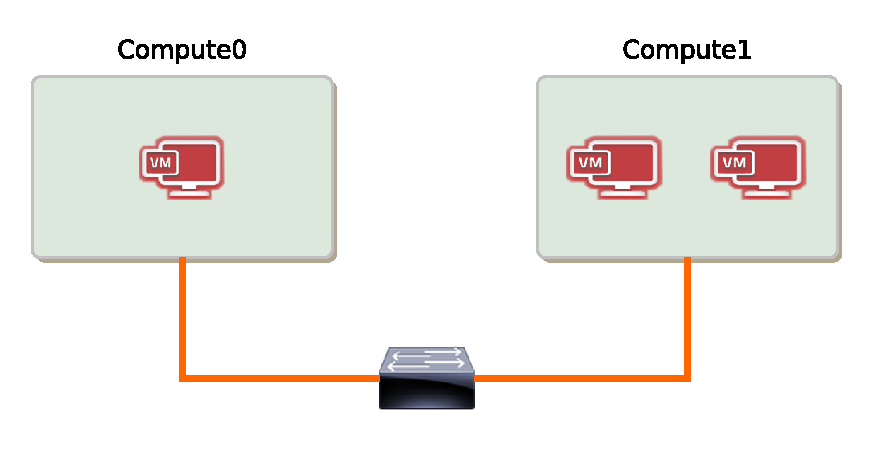
\includegraphics[width=0.8\textwidth]{diagrama.pdf}
    \caption{Esta es una figura que latex decide donde colocar (floating) en el documento.}
    \label{fig:diagrama}
    \end{figure}

  \begin{tabular}{cc}
    Imagen 1 & Imagen 2 \\[2mm]
    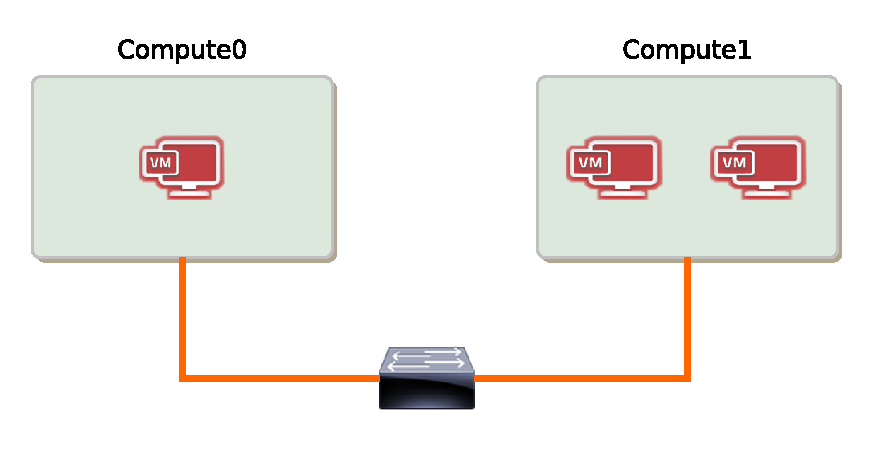
\includegraphics[width=0.4\textwidth]{diagrama.pdf} &  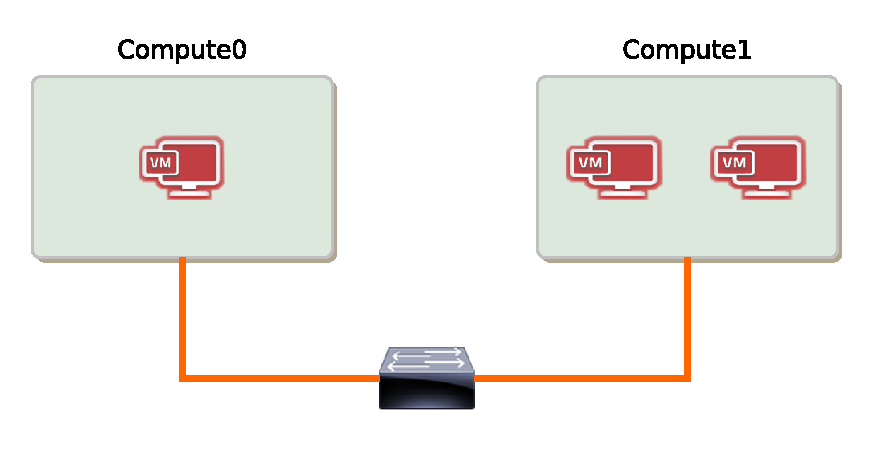
\includegraphics[width=0.4\textwidth]{diagrama.pdf}
  \end{tabular}
  
  Este es un ejemplo de una tabla:
  
  \begin{tabular}{|l|c|}
    \hline
    Columna 1 & Columna 2 \\ \hline
    1 & 2 \\ \hline
  \end{tabular}


  \vspace*{1cm}
  O la misma tabla centrada:

  \begin{center}
    \begin{tabular}{|l|c|}
      \hline
      Columna 1 & Columna 2 \\ \hline
      1 & 2 \\ \hline
    \end{tabular}
  \end{center}

  Para generar el fichero PDF:
  
  \begin{lstlisting}{language=bash}
    pdflatex ejemplo-memoria.tex
    bibtex ejemplo-memoria
    pdflatex ejemplo-memoria.tex
\end{lstlisting}

  También se puede usar \texttt{latexmk} que automáticamente regenera la bibliografía.
  \begin{lstlisting}{language=bash}
    latexmk -pdf ejemplo-memoria.tex
\end{lstlisting}

  

\addcontentsline{toc}{chapter}{Bibliografía}
\bibliographystyle{unsrt}
\bibliography{bib/bibliografia}




\end{document}

%%% Local Variables:
%%% mode: latex
%%% TeX-master: t
%%% End:
